\chapter{Models of the sources of radiation}\label{radiation}
FAINA allows to evaluate electromagnetic radiation from sources with various type of particle distributions and different parameters such as magnetic fiels, number density and other. In this chapter we describe creating various types of radiation sources.

\section{Particle distributions}

Crucial parameter for evaluation of any type of radiation is a distribution function of emitting particles. In the FAINA code abstract class ParticleDistribution and derived classes are used for representation of distributions. Public methods of class ParticleDistribution are listed in Table \ref{ParticleDistribution}:

\begin{small}
		\topcaption{Public methods of ParticleDistribution class}
		\label{ParticleDistribution}
		
		\begin{xtabular}{|p{0.45\textwidth}|p{0.55\textwidth}|}
			\hline
			\textbf{ParticleDistribution} & abstract class for particle distributions\\
			\hline
			double distribution(const double\& energy, const double\& mu, const double\& phi) & returns probability density function in polar coordinates with given energy, cosinus of polar angle and azimutal angle, normalized to the particles number density \\
			\hline
			virtual double distributionNormalized(const double\& energy, const double\& mu, const double\& phi) & virtual method, returns probability density function in polar coordinates with given energy, cosinus of polar angle and azimutal angle, normalized to unity\\
			\hline
			virtual double getMeanEnergy() & virtual method, returns mean energy of particles in distribution\\
			\hline
			double getConcentration() & returns particles number density\\
			\hline
			void resetConcentration(const double\& concentration) & changes number density to the given value\\
			\hline
		\end{xtabular}
\end{small}

For creating a distribution object you need some inherited class. Inheritance tree of ParticleDistribution splits into two big branches - PhotonDistribution for distribution of photons, and MassiveParticleDistribution - for massive particles. Scheme of class hierarchy is shown in Figure  \ref{particleDistribution0}. 

\begin{figure}
	\centering
	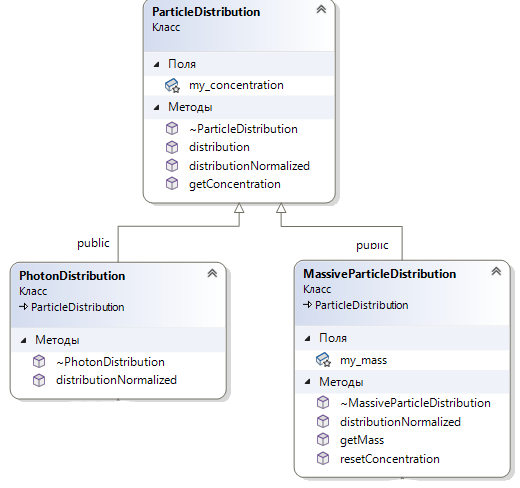
\includegraphics[width=8.5 cm]{./fig/particleDistribution0.png} 
	\caption{Two branches of inheritance tree of ParticleDIstribution}
	\label{particleDistribution0}
\end{figure}

It is important to note, that photons distributions are not used to represent results of evaluation of electromagnetic radiation. They are necessary only as input parameter for evaluation of inverse Compton scattering. Class PhotonDistribution is only an interface and has not its own specific methods. Class MassiveParticleDistribution is also abstract, but his methods are listed in Table \ref{MassiveParticleDistribution}	
\begin{small}
		\topcaption{Public methos of MassiveParticleDistribution class}
		\label{MassiveParticleDistribution}
		
			\begin{xtabular}{|p{0.45\textwidth}|p{0.55\textwidth}|}
				\hline
				\textbf{MassiveParticleDistribution} & abstract class for massive particles distribution\\
				\hline
				virtual double minEnergy() & virtual method, returns the lowest possible energy of particle in this distribution\\
				\hline
				virtual double maxEnergy() & 
				virtual method, returns the upper limit of energy of particle in this distribution. NOTE that if upper limit of energy is infinite, this method returns negative number\\
				\hline
				double getMass() & returns mass of single particle \\
				\hline
			\end{xtabular}
		\end{small}
\subsection{Photon distributions}

Abstract class PhotonDistribution has following derived class: abstract PhotonIsotropicDistribution, which represented isotopic distributions and some non-abstract classes: PhotonPlankDirectedDistribution, which represent photons with Plank distribution with respect to energy, but collimated in some solid angle, and CompoundPhotonDistribution, which is usefull for sum of several arbitrary photon distributions.

Class PhotonIsotropicDistribution again has its own inherited classes. It is a PhotonPowerLawDistribution for powerlaw distribution, PhotonPlankDistribution for Plank distributions, PhotonMultiPlankDistribution for sum of several Plank distributions and PhotonMonoenergeticDistribution for isotropic photons with same energy. Class hoerarchy of photon distributions is presented in Figure \ref{photonDistribution}.

\begin{figure}
	\centering
	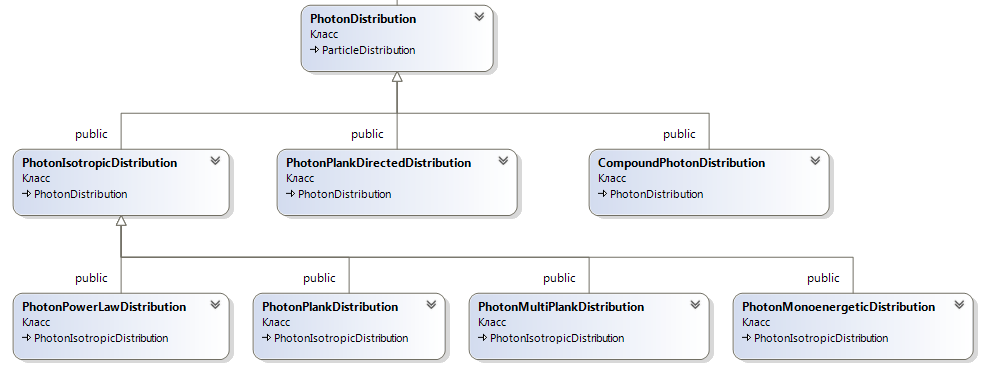
\includegraphics[width=10.5 cm]{./fig/photonDistribution2.png} 
	\caption{Class hierarchy of photon distributions}
	\label{photonDistribution}
\end{figure}

Methods of PhotonDistribution and it's inherited classes are listed in Table \ref{photonDistributionMethods}. NOTE, that metods distributionNormalized(const double\& energy) and distribution(const double\& energy) are not distribution with respect to energy, but just full distribution with dropped angular arguments. So to obtain distribution with respect to energy one should multiply result of this functions by $4\pi$.


\begin{small}
	\topcaption{Public methods of PhotonDistribution class and derived classes}
	\label{photonDistributionMethods}
	\begin{xtabular}{|p{0.45\textwidth}|p{0.55\textwidth}|}
				\hline
				\textbf{PhotonDistribution} & abstract interface for photon distributions\\
				\hline
				\textbf{PhotonIsotropicDistribution} & abstract class for isotropic distributions of photons\\
				\hline
				double distribution(const double\& energy) & returns probability density function in polar coordinates with dropped angular arguments (normalized to the number density divided by $4\pi$)\\
				\hline
				virtual double distributionNormalized(const double\& energy) & virtual method, returns probability density function in polar coordinates with dropped angular arguments (mormalized to the $1/4\pi$)\\
				\hline
				void writeDistribution(const char* fileName, int Ne, const double\& Emin, const double\& Emax) & writes distribution into given file as to columns - energy and distribution from Emin to Emax with Ne logarithmically distributed points\\
				\hline
				\textbf{PhotonPowerLawDistribution} & class representing powerlaw distribution of photons\\
				\hline
				PhotonPowerLawDistribution(const double\& index, const double\& E0, const double\& concentration) & constructor, creates distribution with given power-law index p such as $F(E)~1/E^p$, starting energy and number density \\
				\hline
				double getIndex() & returns power-law index\\
				\hline
				double getE0() & returns starting energy of distribution\\
				\hline
				\textbf{PhotonPlankDistribution} & class representing Plank distribution\\
				\hline
				PhotonPlankDistribution(const double\& temperature, const double\& amplitude) & constructor, creates distribution with given temperature and amplitude - relation of number density to the number density of photons in equilibrium black-body radiation\\
				\hline
				static PhotonPlankDistribution* getCMBRadiation() & static method, returns object representing Cosmic Microwave Background Radiation (temperature $2.725~\rm K$, amplitude $1$)\\
				\hline
				double getTemperature() & returns temperature of distribution\\
				\hline
				\textbf{PhotonMultiPlankDistribution} & class representing sum of several Plank distributions\\
				\hline
				PhotonMultiPlankDistribution(int N, const double* const temperatures, const double* const amplitudes) & constructor, creates distribution constisting of N plank distributions with given temperatures and amplitudes\\
				\hline
				static PhotonMultiPlankDistribution* getGalacticField() & static method, returns object representing mean Galactic photon field described in \cite{Mathis1983}. This distribution consists of five plank components with temperatures $2.725K, 20K, 3000K, 4000K, 7000K$ and amplitudes $1.0, 4\cdot10^{-4}, 4\cdot10^{-13}, 1.65\cdot10^{-13}, 1.0\cdot10^{-14}$ respectively\\
				\hline
				\textbf{PhotonMonoenergeticDistribution} & class representing population of isotropic photons with close energy\\
				\hline
				PhotonMonoenergeticDistribution(const double\& Energy, const double\& halfWidth, const double\& concentration) & constructor, creates object with given mean energy, half-width of uniform distribution around mean energy and number density\\
				\hline
				\textbf{CompoundPhotonDistribution} & class representing sum of several arbitrary distributions\\
				\hline
				CompoundPhotonDistribution(int N, PhotonDistribution** distributions) & constructor, creates distribution consisting of N arbitrary distributions\\
				\hline
				CompoundPhotonDistribution( PhotonDistribution* dist1, PhotonDistribution* dist2) & constructor, creates distribution which is sum of two given distributions\\
				\hline
				CompoundPhotonDistribution( PhotonDistribution* dist1, PhotonDistribution* dist2, PhotonDistribution* dist3) & constructor, creats distribution which is sum of three given distributions\\
				\hline
				\textbf{PhotonPlankDirectedDistribution} & class representing distribution which is Plank-like with respect to energy, but collimated into given direction\\
				\hline
				PhotonPlankDirectedDistribution(const double\& temperature, const double\& amplitude, const double\& theta0, const double\& phi0, const double\& deltaTheta) & constructor, creates distribution with given temperature, amplitude, angles determining mean direction of photons and half-width angle of cone in which photons propagate\\
				\hline
				double getTemperature() & return temperature of distribution\\
				\hline
	\end{xtabular}
\end{small}

User can define other photons distribution, creating class inherited from PhotonDistribution or PhotonIsotropicDistribution and overriding virtual method distributionNormalized.


\subsection{Distributions of massive particles}
Distributions of massive particles are represented by class MassiveParticleDistribution and inherited classes. Similarly to the photon distributions, isotropic distrinutions are important type, represented by class
MassiveParticleIsotropicDistribution. This class also has methods distributionNormalized(const double\& energy) and distribution(const double\& energy), which are not distribution with respect to energy, but just full distribution with dropped angular arguments. So to obtain distribution with respect to energy one should multiply result of this functions by $4\pi$.

Abstract class of isotropic distributions has seven inherited classes for specific distributions: MassiveParticlePowerLawDistribution - for power-law distributions, MassiveParticleBrokenPowerLawDistribution - for double power-law distibutions with knee, MassiveParticlePowerLawCutoffDistribution - for power-law distributions with exponential cutoff, MassiveParticleMaxwellDistribution - for non-relativistic maxwellian distribution (but it use full energy, including rest energy), MassiveParticleMaxwellJuttnerDistribution - for Maxwell
-Juttner distribution, MassiveParticleTabulatedIsotropicDistribution - for arbitrary distributions, described with array of values and MassiveParticleMonoenergeticDistribution - for beam of particles with close energies. Also there are six anisotropic distributions, implemented in the code. MassiveParticleTabulatedPolarDistribution - for tabulated distribution with dependence on energy and polar angle, MassiveParticleAnisotropicDistribution - for arbitrary tabulated anisotropic distributions, MassiveParticleMonoenergeticDirectedDistribution - for distributions represented narrow beam of particles with close energies, MassiveParticleMovingDistribution - for transformation the distributions from one frame to another, CompoundMassiveParticleDistribution - for sum of arbitraty distributions and CompoundWeightedMassiveParticleDistribution - for weighted sum of arbitrary distributions. In some cases operating with relative weghts of distributions is more useful than with absolute concentrations. Class hierarchy of distributions of massive particles is shown in Figure \ref{massiveDistribution}.


\begin{figure}[h]
	\centering
	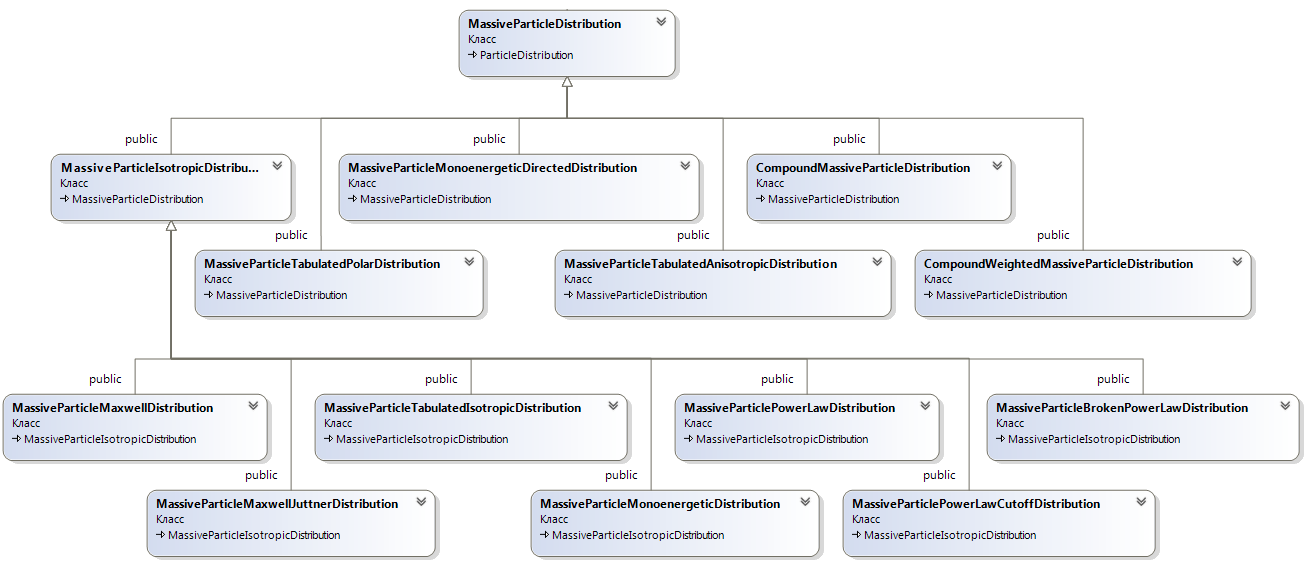
\includegraphics[width=14.5 cm]{./fig/massiveParticleDistribution2.png} 
	\caption{Class hierarchy of massive particles distributions}
	\label{massiveDistribution}
\end{figure}

public methods of classes for massive particle distributions are listed in Table \ref{MassiveParticleMethods}. User can define his own specific distributions, creating class inherited from MassiveParticleDistribution or MassiveParticleIsotropicDistribution.

\begin{small}
	\topcaption{Public methods of classes derived from MassiveParticleDistribution }
	\label{MassiveParticleMethods}
	\begin{xtabular}{|p{0.57\textwidth}|p{0.43\textwidth}|}				
		\hline
		\textbf{MassiveParticleIsotropicDistribution} & Abstract class for isotropic distributions of massive particles\\
		\hline
		double distribution(const double\& energy) & returns probability density function in polar coordinates with dropped angular arguments (normalized to the number density divided by $4\pi$)\\
		\hline
		virtual double distributionNormalized(const double\& energy) & virtual method, returns probability density function in polar coordinates with dropped angular arguments (mormalized to the $1/4\pi$)\\
		\hline
		void writeDistribution(const char* fileName, int Ne, const double\& Emin, const double\& Emax) &writes distribution into given file as to columns - energy and distribution from Emin to Emax with Ne logarithmically distributed points\\
		\hline
		double distributionNormalizedWithLosses( const double\& energy, const double\& lossRate, const double\& time) & returns a distribution which evaluted till time t via synchrotron losses with equation $f_t(E)=f\left(\frac{E}{1-E l t}\right)\cdot\frac{1}{\left(1- E l t\right)^2}$ and loss rate $l = 4e^4 B^2 /9m^4 c^7$\\
		\hline
		\textbf{MassiveParticlePowerLawDistribution} & class representibg power-law distribution\\
		\hline
		MassiveParticlePowerLawDistribution( const double\& mass, const double\& index, const double\& E0, const double\& concentration) & cobstructor, creates distribution with given particle mass, power-law index, starting energy and concentration\\
		\hline
		double getIndex() &returns power-law index\\
		\hline
		double getE0() & returns starting energy of distribution\\
		\hline
		\textbf{MassiveParticleBrokenPowerLawDistribution} & class representing double power-law distribution with knee\\
		\hline
		MassiveParticleBrokenPowerLawDistribution( const double\& mass, const double\& index1, const double\& index2, const double\& E0, const double\& Etran, const double\& concentration) & constructor, creates distribution with given particle mass, power-law indexes at low and high energies, starting energy, energy of transition from one index to another and concentration\\
		\hline
		double getIndex1() & returns power-law index at low energies\\
		\hline
		double getIndex2() & returns power-law index at high energies\\
		\hline
		double getE0() & returns starting energy of distribution\\
		\hline
		double getEtran() & returns energy of transition fron one index to another\\
		\hline
		\textbf{MassiveParticlePowerLawCutoffDistribution} & class representing power-law distribution with exponential cutoff\\
		\hline
		MassiveParticlePowerLawCutoffDistribution(const double\& mass, const double\& index, const double\& E0, const double\& beta, const double\& Ecut, const double\& concentration) & constructor, creates distribution with given particle mass, power-law index, starting energy, power of cutoff and cutoff energy and concentration $F(E)\propto (E/E_0)^{-index}\cdot\exp(-(E/E_{cut})^\beta)$\\
		\hline
		double getIndex() & returns power-law index \\
		\hline
		double getBeta() & returns cutoff power parameter \\
		\hline
		double getE0() & returns starting energy of distribution\\
		\hline
		double getEcutoff() & returns cutoff energy\\
		\hline
		\textbf{MassiveParticleMaxwellDistribution} & class representing non-relativistic maxwellian distribution\\
		\hline
		MassiveParticleMaxwellDistribution( const double\& mass, const double\& temperature, const double\& concentration) & creates distribution with given particles mass, temperature and concentration\\
		\hline
		double getTemperature() & returns temperature\\
		\hline
		\textbf{MassiveParticleMaxwellJuttnerDistribution} & class representing Maxwell-Juttner distribution\\
		\hline
		MassiveParticleMaxwellJuttnerDistribution( const double\& mass, const double\& temperature, const double\& concentration) & creates distribution with given particle mass, temperature and concentration\\
		\hline
		double getTemperature() & returns temperature\\
		\hline
		\textbf{MassiveParticleTabulatedIsotropicDistribution} & class for tabulated isotropic distribution\\
		\hline
		MassiveParticleTabulatedIsotropicDistribution( const double\& mass, const char* fileName, const int N, const double\& concentration, DistributionInputType inputType) & constructor, creates distribution with given mass and concentraion, reading table with N lines from given file. inpuType - enum variable determining in which coordinates distribution is defined in file\\
		\hline
		MassiveParticleTabulatedIsotropicDistribution( const double\& mass, const char* energyFileName, const char* distributionFileName, const int N, const double\& concentration, DistributionInputType inputType) & constructor, creates distribution with given mass and concentraion, reading Nx2 table with from two given files. inpuType - enum variable determining in which coordinates distribution is defined in files\\
		\hline
		MassiveParticleTabulatedIsotropicDistribution( const double\& mass, const double* energy, const double* distribution, const int N, const double\& concentration, DistributionInputType inputType) & constructor, creates distribution with given mass and concentraion, reading two data columns from given arrays. inpuType - enum variable determining in which coordinates distribution is defined in arrays\\
		\hline
		int getN() & returns number of grid points in distribution array\\
		\hline
		double rescaleDistribution(const double\& k) & rescales distribution through the energy axis using fourmula $E' = mc^2 + k\cdot(E-mc^2)$, $F(E')=F(E)/k$. It may be useful when e.g. distribution of electrons is obtained by numerical code with increased electron mass\\
		\hline
		void addPowerLaw( const double\& Epower, const double\& index) & replaces the tail of distribution with power-law distribution with given spectral index starting from Epower. Also renorms distribution\\
		\hline
		\textbf{MassiveParticleMonoenergeticDistribution} & class representing population of isotropic particles with close energy\\
		\hline
		MassiveParticleMonoenergeticDistribution(const double\& mass, const double\& Energy, const double\& halfWidth, const double\& concentration) & constructor, creates distribution with given particle mass, mean energy, half-width of uniform distribution around mean energy and number density\\
		\hline 
		\textbf{MassiveParticleTabulatedPolarDistribution} & class for tabulated distribution with dependence on energy and polar angle\\
		\hline
		MassiveParticleTabulatedPolarDistribution( const double\& mass, const char* energyFileName, const char* muFileName, const char* distributionFileName, const int Ne, const int Nmu, const double\& concentration, DistributionInputType inputType) & constuctor, creates distribution with given particle mass and concentration, reading it from files with energy grid points, angular grid points and distribution. inpuType - enum variable determining in which coordinates distribution is defined in files\\
		\hline
		MassiveParticleTabulatedPolarDistribution( const double\& mass, const double* energy, const double* mu, const double** distribution, const int Ne, const int Nmu, const double\& concentration, DistributionInputType inputType) & constuctor, creates distribution with given particle mass and concentration, using arrays with energy grid points, angular grid points and distribution. inpuType - enum variable determining in which coordinates distribution is defined in arrays\\
		\hline
		int getNe() & returns number of energy grid points in distribution array\\
		\hline
		int getNmu() & returns number of polar angle grid points in distribution array\\
		\hline
		void double rescaleDistribution(const double\& k) & 
		rescales distribution through the energy axis using fourmula $E' = mc^2 + k\cdot(E-mc^2)$, $F(E',\mu)=F(E,\mu)/k$. It may be useful when e.g. distribution of electrons is obtained by numerical code with increased electron mass\\
		\hline
		\textbf{MassiveParticleTabulatedAnisotropicDistribution} & class for arbitrary tabulated distribution\\
		\hline
		MassiveParticleTabulatedAnisotropicDistribution( const double\& mass, const char* energyFileName, const char* muFileName, const char* distributionFileName, const int Ne, const int Nmu, const int Nphi, const double\& concentration, DistributionInputType inputType) & constuctor, creates distribution with given particle mass and concentration, reading it from files with energy grid points, angular grid points and distribution. Grid with respect to azimuthal angle considered uniform and depends only on number of drid points Nphi. inpuType - enum variable determining in which coordinates distribution is defined in files\\
		\hline
		MassiveParticleTabulatedAnisotropicDistribution( const double\& mass, const double* energy, const double* mu, const double*** distribution, const int Ne, const int Nmu, const int Nphi, const double\& concentration, DistributionInputType inputType) & constuctor, creates distribution with given particle mass and concentration, using arrays with energy grid points, angular grid points and distribution. Grid with respect to azimuthal angle considered uniform and depends only on number of drid points Nphi. inpuType - enum variable determining in which coordinates distribution is defined in arrays\\
		\hline
		int getNe() & returns number of energy grid points in distribution array\\
		\hline
		int getNmu() & returns number of polar angle grid points in distribution array\\
		\hline
		int getNphi() & returns number of azimuthal angle grid points in distribution array\\
		\hline
		void rescaleDistribution(const double\& k) & rescales distribution through the energy axis using fourmula $E' = mc^2 + k\cdot(E-mc^2)$, $F(E',\mu, \phi)=F(E,\mu, \phi)/k$. It may be useful when e.g. distribution of electrons is obtained by numerical code with increased electron mass\\
		\hline
		\textbf{MassiveParticleMonoenergeticDirectedDistribution} & class representing narrow beam of particles with close energies\\
		\hline
		MassiveParticleMonoenergeticDirectedDistribution( const double\& mass, const double\& Energy, const double\& halfWidth, const double\& concentration, const double\& theta0, const double\& phi0, const double\& deltaTheta) & constructor, creates distribution with given particle mass, mean energy, half-width of uniform distribution around the mean energy, polar and azimuthal angles determining direction of mean velocity and half-width angle of velocity cone\\
		\hline
		\textbf{MassiveParticleMovingDistribution} & class transforming distribution from one frame to another\\
		\hline
		MassiveParticleMovingDistribution( MassiveParticleDistribution* distribution, const double\& velocity) & constructor, transforms the given distribution from the frame with givem velocity along z-axis to the lab frame\\
		\hline
		\textbf{CompoundMassiveParticleDistribution} & class representing distribution as sum of other distributions\\
		\hline
		CompoundMassiveParticleDistribution( int N, MassiveParticleDistribution** distributions) & constructor, creates distribution which is sum of given distributions\\
		\hline
		CompoundMassiveParticleDistribution( MassiveParticleDistribution* dist1, MassiveParticleDistribution* dist2) & constructor, creates distribution which is sum of two given distributions\\
		\hline
		CompoundMassiveParticleDistribution( MassiveParticleDistribution* dist1, MassiveParticleDistribution* dist2, MassiveParticleDistribution* dist3) & constructor, creates distribution which is sum of three given distributions\\
		\hline
		\textbf{CompoundWeightedMassiveParticleDistribution} & class representing distribution as weighted sum of other distributions\\
		\hline
		CompoundWeightedMassiveParticleDistribution( int N, const double* weights, MassiveParticleDistribution** distributions) & constructor, creates distribution which is sum of given distributions with given weights\\
		\hline
		CompoundWeightedMassiveParticleDistribution( MassiveParticleDistribution* dist1, const double\& w1, MassiveParticleDistribution* dist2, const double\& w2) & constructor, creates distribution which is sum of two given distributions with given weights\\
		\hline
		CompoundWeightedMassiveParticleDistribution( MassiveParticleDistribution* dist1, const double\& w1, MassiveParticleDistribution* dist2, const double\& w2, MassiveParticleDistribution* dist3, const double\& w3) & constructor, creates distribution which is sum of three given distributions with given weights\\
		\hline
		
	\end{xtabular}
\end{small}

\subsection{Reading distributions from file}
Classes for tabulated distribution, such as MassiveParticleTabulatedIsotropicDistribution, have constructors allowing to read distributions from files. It should be text files with tables of data, and format of data can be different. For determining data format there is enumerable type DistributionInputType with five possible values:

\begin{itemize}
	\item ENERGY\_FE - input file contains full energy in CGS units and distribution function $F(E)$
	\item ENERGY\_KIN\_FE - input file contains kinetic energy in CGS units and distribution function $F(E_{kin})$
	\item GAMMA\_FGAMMA - input file contains lorentz-factor and distribution function with respect to it $F(\gamma)$
	\item GAMMA\_KIN\_FGAMMA - input file contains reduced lorentz-factor ($\gamma - 1$) and distribution function with respect to it $F(\gamma-1)$
	\item MOMENTUM\_FP - input file contains momentum in CGS units and distribution function with respect to it $F(p)$
\end{itemize}

Regardless of input file format, distribution function would be transformed to the units energy vs distribution $F(E)$. Example of reading distribution from file is given below

\begin{lstlisting}[language=c++]
	double electronConcentration = 1.0;
	int N = 100;
	MassiveParticleIsotropicDistribution* distribution = new
	MassiveParticleTabulatedIsotropicDistribution(massElectron,
	"energy.dat", "distribution.dat", N, electronConcentration,
	DistributionInputType::ENERGY_FE);
\end{lstlisting}

Class MassiveParticleDistributionFactory is implemented for simplicity of reading distributions from files in complicated cases. It has several similar static methods allowing to read array of distribution from set of numerated files. It can be useful in cases when distribution function depends on some external parameter which varies inside the radiation source. Example of reading array of ten distributions of electrons from files, named "Fe0.dat"\ , "Fe1.dat"\ etc., consisting of two columns - loerntz-factor and distribution function, and adding power-law tail with index 3, starting from energy $10 m_e c^2$, calling one function is given below

\begin{lstlisting}[language=c++]
	double electronConcentration = 1.0;
	int Nenergy = 100;
	int Ndistribution = 100;
	double powerLawEnergy = 100*me_c2;
	double index = 3.0;
	MassiveParticleIsotropicDistribution** distributions = 
	MassiveParticleDistributionFactory::
	readTabulatedIsotropicDistributionsAddPowerLawTail(
	massElectron, "./input/Fe", ".dat", Ndistribution, 
	DistributionInputType::GAMMA_FGAMMA, electronConcentration, Nenergy,
	powerLawEnergy, index);
\end{lstlisting}

Also it is possible to create tabulated distributions not by reading them from files, but from arrays, which can be generated by user with any suitable method.

\section{Radiation sources}

To evaluate electromagnetic radiation with FAINA code user should create object, representing radiation source. It allows to take into account geomtry of the source, it's inhomogenuity and other features.

There are two types of radiation sources - sources without time dependency, represented with class RadiationSource, and cources depending on time, represented with class RadiationTimeDependentSource. This two classes are not related with each other through inheritance, but the object of class RadiationTimeDependentSource contains the object of class RadiationSource inside. Diagram of class hierarchy of radiation sources is shown in Figure \ref{radiationSource}.

\begin{figure}[h]
	\centering
	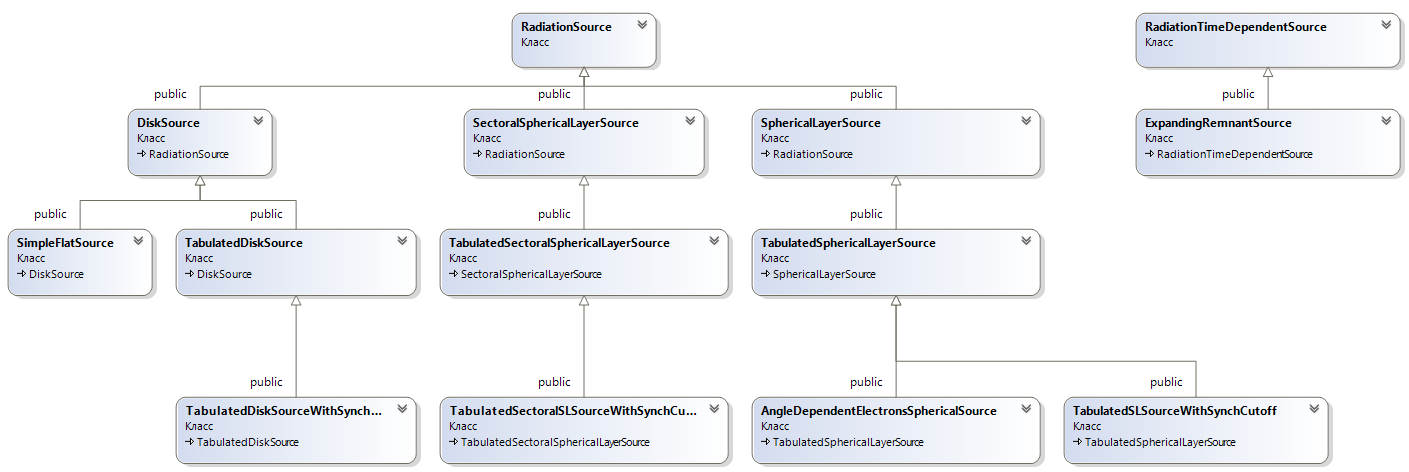
\includegraphics[width=14.5 cm]{./fig/radiationSource2.png} 
	\caption{class hierarchy of radiation sources}
	\label{radiationSource}
\end{figure}

\subsection{Radiation sources without time dependency}\label{sourcesSection}
Radiation sources without time dependency are represented with abstract class RadiationSourse and it's derived classes. All sources models uses cylinrical grid with z axis along line of sight. This allows easily integrate through z-axis taking into accound absorption processes. Difference of the real shape of the source from discrete shape of a grid is compensated with filling factor of every grid cell. It represent fraction of cell volume which is located inside the source. Model of the source with geometry of spherical layer is shown in Figure \ref{sphericalLayer}. Colour shows filling factors of each cell.

\begin{figure}[h]
	\centering
	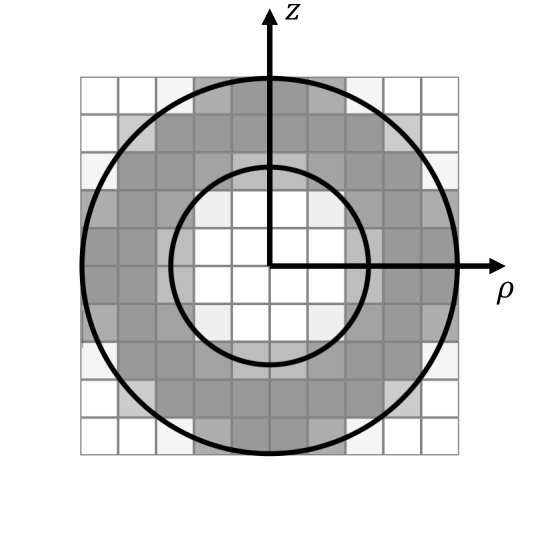
\includegraphics[width=10.5 cm]{./fig/sphericalSource.png} 
	\caption{Model of the source with spherical layer geometry in the cylindrical grid. Colour shows fraction of cell volume which is located inside the source.}
	\label{sphericalLayer}
\end{figure}

Radiation sources have following parameters, that can vary in different grid cells: concentration of emmitting particles, their distribution functions, magnetic field and it's orientation angles. Also distance to the observer is important parameter of the source.

Class RadiationSource has three abstract derived classes: DiskSource - for the sources with shape of a disk with axis along line of sight, SphericalLayerSource - for sources with shape of a spherical layer and SectoralSphericalLayerSource - for sources with shape of spherical layer restricted with some azimutal angle range, and also with minimum cylindrical radius limit. The last one is useful when real source is a prolonged object observed with high resolution, and some features of radiation from different regions of the source are studied.

Sources with disk shape have three specific implementations: SimpleFlatSource - homogenous disk consisting of only one grid cell with given parameters, TabulatedDiskSource - inhomogenous disk in wich all parameters are tabulated on the spatial grid, and TabulatedDiskSourceWithSynchCutoff, which is inherited from previous one and allows to take into account synchrotron losses of emitting particles during their propagation inside the sourse. In this source model particles distribution is suppose to be generated on the upper face of disk, representing shock wave, and then particles are moving via convection inside the source. Evolution of the distribution function is described with equation:

\begin{equation}
	f_l(E)=f\left(\frac{E}{1-4e^4 B^2 E~l/9m^4 c^7 v}\right)\cdot\frac{1}{\left(1-4e^4 B^2 E~l/9m^4 c^7 v\right)^2}
\end{equation}

where $f(E)$ generated distribution function, $E$ - energy of the particle, $B$ - magnetic field, $l$ - distance from given point to the upper face, $v$ - velocity of convection movement, $e$ - absolute value of particle charge, $m$ - particle mass, $c$ - speed of light.

Sources with shape of spherical layers have following implementations: TabulatedSphericalSource, in wich all parameters are tabulated on the spatial grid and two classes derived from it  TabulatedSLSourceWithSynchCutoff and AngleDependentElectronsSphericalSource. First of them allows to take into account synchrotron losse, like it was done in TabulatedDiskSourceWithSynchCutoff, but in this case distribution is generated on the outer spherical surface, and the second is useful for important case in astrophysics when distribution function of emitting particles is dependent on inclination angle of magnetic field to the direction of shock propagation \cite{SironiSpitkovsky2009pair, GuoSironi2014_1,Crumley2019, Romansky2018}. In AngleDependentElectronsSphericalSource such parameters as number density, magnetic field and it's orintation angles are tabulated on the spatial grid, while distribution function is tabulated with respect of inclination angle of magnetic field to the shock, which is considered spherically symmetrical and propagates along radius.

Sources with shape of sector of spherical layer has following implementations: TabulatedSectoralSphericalLayerSource, in wich all parameters are tabulated on the spatial grid and derived from it TabulatedSectoralSLSourceWithSynchCutoff, taking into account synchrotron energy losses like it was done in TabulatedSLSourceWithSynchCutoff.

Public methods of classes for radiation sources are listed in the Table \ref{sourceMethods1}.

\begin{small}
	\topcaption{Public methods of classes for time independent radiation sources}
	\label{sourceMethods1}
	\begin{xtabular}{|p{0.5\textwidth}|p{0.5\textwidth}|}
		\hline
		\textbf{RadiationSource} & abstract class for radiation sources\\
		\hline
		virtual double getMaxRho() & virtual method, returns upper boundary of the source at the cylindrical radius\\
		\hline
		virtual double getMinRho() & virtual method, returns lower boundary of the source at the cylindrical radius\\
		\hline
		virtual double getMinZ() & virtual method, returns lower boundary of the source at the z axis\\
		\hline
		virtual double getMaxZ() & virtual method, returns upper boundary of the source at the z axis\\
		\hline
		virtual double getMaxB() & virtual method, returns maximal magnetic field in the source\\
		\hline
		virtual double getAverageSigma() & virtual method, returns average magnetization $\sigma=\frac{B^2}{4\pi n m_p c^2}$\\
		\hline
		virtual double getAverageConcentration() & virtual method, returns average number density\\
		\hline
		virtual double getRho(int irho) & virtual method, returns cylindrical radius of the cell with number irho through the radial axis\\
		\hline
		virtual double getZ(int iz)& virtual method, returns z coordinate of the cell with number iz through the z axis\\
		\hline
		virtual double getPhi(int iphi)& virtual method, returns azimutal angle of the cell with iphi number through the azimutal coordinate\\
		\hline
		virtual int getRhoIndex(const double\& rho)& virtual method, returns radial number of cell containing given radial coordinate\\
		\hline
		virtual bool isSource(int irho, int iphi)& virtual method, return boolean value defining are cells with given radial and azimutal numbers part of the source or not. It is useful for modeling of sources with complex geometry \\
		\hline
		int getNrho() & returns number of grid points through the radial axis\\
		\hline
		int getNz() & returns number of grid points through the z axis\\
		\hline
		int getNphi() & returns number of grid points twith respect to the azimutal angle\\
		\hline
		double getDistance() & returns distance to the source\\
		\hline
		virtual getArea(int irho) & virtual method, returns average area of cross-section of part of the cell, filled with the source matter\\
		\hline
		virtual getLength(int irho, int iz, int iphi) & virtual method, returns average thickness of the part of the source, filled with the source matter\\
		\hline
		getVolume(int irho, int iz, int iphi) & returns volume of the part of the cell, filled with source matter. This method is consistent with getArea and getLength, and returns their product\\
		\hline
		virtual getB(int irho, int iz, int iphi) & virtual method, returns magnetic filled in given cell\\
		\hline
		virtual getConcentration(int irho, int iz, int iphi) & virtual method, returns number density in given cell\\
		\hline
		virtual getSinTheta(int irho, int iz, int iphi) & virtual method, returns sinus of angle between magnetic field and line of sight in given cell\\
		\hline
		virtual void getVelocity(int irho, int iz, int iphi, double\& velocity, double\& theta, double\& phi) &
		virtual method, returns velocity in given cell, and polar and azimutal angles for it's direction\\
		\hline
		virtual getTotalVolume() & virtual method, returns total volume of the source\\
		\hline
		virtual resetParameters(const double* parameters, const double* normalizationUnits) &
		virtual method, reseting parameters of the source. Lists of parameters are different for different types of sources. Method takes for input array of parameters in normalized units, and array of normalization conctants. This method for example is used for fitting modelled radiation to the observational data and optimization such parameters as magnetic field, number density and others. Also it is used to model time evolution of the source\\
		\hline
		virtual getParticleDistribution(int irho, int iz, int iphi) & virtual method, returns emitting particles distribution in given cell\\
		\hline
		\textbf{DiskSource} & abstract class for sources with shape of a disk\\
		\hline
		\textbf{SimpleFlatSource} & class for homogenous disk sources\\
		\hline
		SimpleFlatSource( MassiveParticleDistribution* electronDistribution, const double\& B, const double\& theta, const double\& rho, const double\& z, const double\& distance, const double\& velocity = 0) & constructor, creates rasiation source with given distribution of emitting particles, magnetic field, angle of it's inclination angle to the line of sight, number density, disk radius, thickness, distance to the observer and velocity of the source matter along z axis \\
		\hline
		\textbf{TabulatedDiskSource} & class for disk sources with tabulated parameters\\
		\hline
		TabulatedDiskSource( int Nrho, int Nz, int Nphi, MassiveParticleDistribution* electronDistribution, double*** B, double*** sinTheta, double*** concentration, const double\& rho, const double\& z, const double\& distance, const double\& velocity = 0) & constructor, creates radiation source with given distribution of emitting particles and tabulated magnetic field, it's inclination angle to the line of sight, number density, disk radius, thickness, distance to the observer and velocity of the source matter along z axis\\
		\hline
		TabulatedDiskSource( int Nrho, int Nz, int Nphi, MassiveParticleDistribution* electronDistribution, const double\& B, const double\& sinTheta, const double\& concentration , const double\& rho, const double\& z, const double\& distance, const double\& velocity = 0) & constructor, creates radiation source with given distribution of emitting particles and uniform magnetic field, it's inclination angle to the line of sight, number density, disk radius, thickness, distance to the observer and velocity of the source matter along z axis\\
		\hline
		\textbf{TabulatedDiskSourceWithSynchCutoff} & class for disk sources with tabulated parameters and taking into account synchrotron energy losses\\
		\hline
		TabulatedDiskSourceWithSynchCutoff(int Nrho, int Nz, int Nphi, MassiveParticleDistribution* electronDistribution, double*** B, double*** theta, double*** concentration, const double\& rho, const double\& z, const double\& distance, const double\& downstreamVelocity, const double\& velocity = 0) &
		constructor, creates radiation source with given distribution of emitting particles and tabulated magnetic field, it's inclination angle to the line of sight, number density, disk radius, thickness, distance to the observer convection velocity of emitting particles and velocity of the source matter along z axis\\
		\hline
		TabulatedDiskSourceWithSynchCutoff(int Nrho, int Nz, int Nphi, MassiveParticleDistribution* electronDistribution, const double\& B, const double\& concentration, const double\& theta, const double\& rho, const double\& z, const double\& distance, const double\& downstreamVelocity, const double\& velocity = 0) & given distribution of emitting particles and uniform magnetic field, it's inclination angle to the line of sight, number density, disk radius, thickness, distance to the observer, convection velocity of emitting particles and velocity of the source matter along z axis\\
		\hline
		\textbf{SphericalLayerSource} & abstract class for sources with the shape of spherical layer\\
		\hline
		double getInnerRho() & returns inner radius of spherrical layer\\
		\hline
		\textbf{TabulatedSphericalLayerSource} & class for sources with the shape of spherical layer with tabulated parameters\\
		\hline
		TabulatedSphericalLayerSource(int Nrho, int Nz, int Nphi, MassiveParticleDistribution* electronDistribution, double*** B, double*** sinTheta, double*** concentration, const double\& rho, const double\& rhoin, const double\& distance, const double\& velocity = 0) & constructor, creates radiation source with given distribution of emitting particles and tabulated magnetic field, it's inclination angle to the line of sight, number density, external and internal radii of spherical layer, distance to the observer and velocity of the source matter along radius\\
		\hline
		TabulatedSphericalLayerSource(int Nrho, int Nz, int Nphi, MassiveParticleDistribution* electronDistribution, const double\& B, const double\& concentration, const double\& sinTheta, const double\& rho, const double\& rhoin, const double\& distance, const double\& velocity = 0) &  constructor, creates radiation source with given distribution of emitting particles and uniform magnetic field, it's inclination angle to the line of sight, number density, external and internal radii of spherical layer, distance to the observer and velocity of the source matter along radius\\
		\hline
		\textbf{AngleDependentElectronsSphericalSource} & class for sources with the shape of spherical layer, and dependency of distribution function on inclination of magnetic field to the shock propagation velocity\\
		\hline
		AngleDependentElectronsSphericalSource( int Nrho, int Nz, int Nphi, int Ntheta, MassiveParticleDistribution** electronDistributions, double*** B, double*** sinTheta, double*** phi, double*** concentration, const double\& rho, const double\& rhoin, const double\& distance, const double\& velocity = 0) & constructor, creates radiation source with given arrays of distributions of emitting particles for different inclination angles and tabulated magnetic field, it's inclination angle to the line of sight, number density, external and internal radii of spherical layer, distance to the observer and velocity of the source matter along radius\\
		\hline
		AngleDependentElectronsSphericalSource(int Nrho, int Nz, int Nphi, int Ntheta, MassiveParticleDistribution** electronDistributions, const double\& B, const double\& sinTheta, const double\& phi, const double\& concentration, const double\& rho, const double\& rhoin, const double\& distance, const double\& velocity = 0) & constructor, creates radiation source with given arrays of distributions of emitting particles for different inclination angles and uniform magnetic field, it's inclination angle to the line of sight, number density, external and internal radii of spherical layer, distance to the observer and velocity of the source matter along radius\\
		\hline
		\textbf{TabulatedSLSourceWithSynchCutoff} & class for sources with the shape of spherical layer taking into acount synchrotron energy losses\\
		\hline
		TabulatedSLSourceWithSynchCutoff(int Nrho, int Nz, int Nphi, MassiveParticleDistribution* electronDistribution, double*** B, double*** theta, double*** concentration, const double\& rho, const double\& rhoin, const double\& distance, const double\& downstreamVelocity, const double\& velocity = 0) & constructor, creates radiation source with given distribution of emitting particles and tabulated magnetic field, it's inclination angle to the line of sight, number density, external and internal radii of spherical layer, distance to the observer, convection velocity of emitting particles and velocity of the source matter along radius\\
		\hline
		TabulatedSLSourceWithSynchCutoff(int Nrho, int Nz, int Nphi, MassiveParticleDistribution* electronDistribution, const double\& B, const double\& concentration, const double\& theta, const double\& rho, const double\& rhoin, const double\& distance, const double\& downstreamVelocity, const double\& velocity = 0) & constructor, creates radiation source with given distribution of emitting particles and uniform magnetic field, it's inclination angle to the line of sight, number density, external and internal radii of spherical layer, distance to the observer, convection velocity of emitting particles and velocity of the source matter along radius\\
		\hline
		\textbf{SectoralSphericalLayerSource} & abstract class for sources with shape of sector of spherical layer\\
		\hline
		double getRhoin() & returns internal radius of spherical layer\\
		\hline
		\textbf{TabulatedSectoralSphericalLayerSource} & class for sources with the shape of spherical layer with tabulated parameters\\
		\hline
		TabulatedSectoralSphericalLayerSource(int Nrho, int Nz, int Nphi, MassiveParticleDistribution* electronDistribution, double*** B, double*** theta, double*** concentration, const double\& rho, const double\& rhoin, const double\& minrho, const double\& phi, const double\& distance, const double\& velocity = 0) & constructor, creates radiation source with given distribution of emitting particles and tabulated magnetic field, it's inclination angle to the line of sight, number density, external and internal radii of spherical layer, minimal cylindrical radius, azimutal width of the sector, distance to the observer and velocity of the source matter along radius\\
		TabulatedSectoralSphericalLayerSource(int Nrho, int Nz, int Nphi, MassiveParticleDistribution* electronDistribution, const double\& B, const double\& concentration, const double\& theta, const double\& rho, const double\& rhoin, const double\& minrho, const double\& phi, const double\& distance, const double\& velocity = 0) & constructor, creates radiation source with given distribution of emitting particles and uniform magnetic field, it's inclination angle to the line of sight, number density, external and internal radii of spherical layer, minimal cylindrical radius, azimutal width of the sector, distance to the observer and velocity of the source matter along radius\\
		\hline
		\textbf{TabulatedSectoralSLSourceWithSynchCutoff} & class for sources with the shape of sector of spherical layer taking into account synchrotron losses\\
		\hline
		TabulatedSectoralSLSourceWithSynchCutoff(int Nrho, int Nz, int Nphi, MassiveParticleDistribution* electronDistribution, double*** B, double*** theta, double*** concentration, const double\& rho, const double\& rhoin, const double\& minrho, const double\& phi, const double\& distance, const double\& downstreamVelocity, const double\& velocity = 0) & constructor, creates radiation source with given distribution of emitting particles and tabulated magnetic field, it's inclination angle to the line of sight, number density, external and internal radii of spherical layer, minimal cylindrical radius, azimutal width of the sector, distance to the observer, convection velocity of emitting particles and velocity of the source matter along radius\\
		\hline
		TabulatedSectoralSLSourceWithSynchCutoff(int Nrho, int Nz, int Nphi, MassiveParticleDistribution* electronDistribution, const double\& B, const double\& concentration, const double\& theta, const double\& rho, const double\& rhoin, const double\& minrho, const double\& phi, const double\& distance, const double\& downstreamVelocity, const double\& velocity = 0) & constructor, creates radiation source with given distribution of emitting particles and uniform magnetic field, it's inclination angle to the line of sight, number density, external and internal radii of spherical layer, minimal cylindrical radius, azimutal width of the sector, distance to the observer, convection velocity of emitting particles and velocity of the source matter along radius\\
		\hline
	\end{xtabular}
\end{small}

\subsection{Radiation sources with time dependency}\label{timeDependentSource}

Radiation sources, taking into account time dependency, are represented with abstract class RadiationTimeDependentSource. This class is not derived from RadiationSource, but it contains object of this type as private field for evaluation of radiation at specific time moment. RadiationSource object with parameters corresponding to the given time moment can be obtained with virtual method getRadiationSource. This method uses resetParameters method of RadiationSource to model time evolution, so it is important to make sure that parameters of RadiationSource object are consistent with implementation of getRadiationSource method. In current version of FAINA there is only one implementation of RadiationTimeDependentSource - ExpandingRemnantSource which represents model of expanding spherical supernove remnant. In this model radius of the source is sopposed to change through time with powerlaw dependency $R\propto t^{p_t}$, and magnetic field and number density depend on time as $B\propto1/R^{p_B}$ and $n\propto1/R^{p_n}$. Public methods of classes RadiationTimeDependentSource and ExpandingRemnantSource are listed in Table \ref{sourceTimeDependentMethods1}. User can create his own implementation of RadiationTimeDependentSource for more compliceted models.

\begin{small}
	\topcaption{Public methods of radiation sources with time dependency }
	\label{sourceTimeDependentMethods1}
	\begin{xtabular}{|p{0.5\textwidth}|p{0.5\textwidth}|}
		\hline
		\textbf{RadiationTimeDependentSource} & abstract class for sources with time dependency\\
		\hline
		virtual resetParameters(const double* parameters, const double* normalizationUnits) & virtual method, reseting parameters of the source (not the same as for RadiationSource). Lists of parameters are different for different types of sources. Method takes for input array of parameters in normalized units, and array of normalization conctants. This method for example is used for fitting modelled radiation to the observational data and optimization such parameters as magnetic field, number density and others.\\
		\hline
		virtual getRadiationSource(double\& time, const double* normalizationUnits) & virtual method, returns RadiationSOurce at given time moment. Also needs normaliztion units for source parameters \\
		\hline
		\textbf{ExpandingRemnantSource} & class representing expanding supernove remnant\\
		\hline
		ExpandingRemnantSource(const double\& R0, const double\& B0, const double\& concentration0, const double\& v, const double\& widthFraction, RadiationSource* source, const double\& t0, const double\& radiusPower = 1.0, const double\& Bpower = 1.0, const double\& concentrationPower = 2.0) & constructor, creates expanding source, wight given at moment t0 radius, magnetic field, number density, velocity of expansion, fraction of radius filled with source matter, model of the source and power index of dependencies of radius, magnetic field and number density.\\
		\hline
	\end{xtabular}
\end{small}
